\documentclass[aspectratio=169]{beamer}
\usetheme[block=fill]{metropolis}
\usepackage{tikz}
\usetikzlibrary{shapes.geometric, arrows.meta, positioning, calc}

\title{Building a Reproducible Scholarly Search Toolkit}
\subtitle{Episode 15: The Orchestrator Engine}
\author{Scholar Search Kit}
\date{}

\begin{document}

\begin{frame}[plain]
  \titlepage
\end{frame}

\begin{frame}{Episode Goal}
  \begin{alertblock}{The Goal}
    Build the \texttt{SearchEngine} class that glues all our subsystems (Providers, Rate Limiting, Deduplication) together.
  \end{alertblock}
  \vspace{0.5cm}
  Until now, we have built isolated components. The Orchestrator is the conductor that reads the query, calls the provider, deduplicates the results, and hands them to the exporter.
\end{frame}

\begin{frame}{The Orchestration Flow}
  \begin{center}
  \resizebox{0.9\linewidth}{!}{
  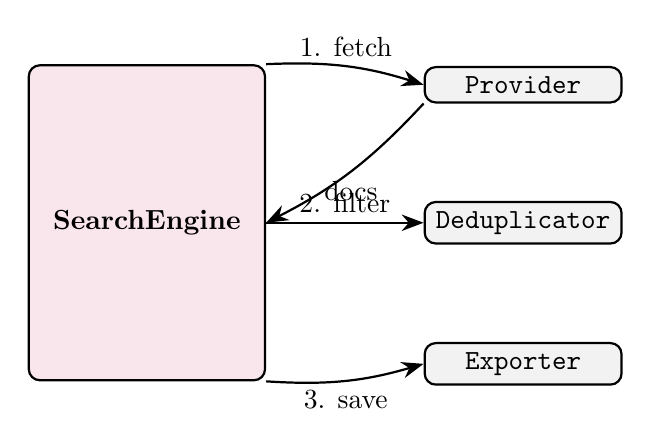
\begin{tikzpicture}[
      node distance=1cm and 1cm,
      comp/.style={rectangle, draw, thick, rounded corners, minimum width=2.5cm, align=center, fill=black!5},
      engine/.style={rectangle, draw, thick, rounded corners, minimum width=3cm, minimum height=4cm, align=center, fill=purple!10},
      arrow/.style={-{Stealth[scale=1.2]}, thick}
    ]
    
    \node[engine] (eng) {\textbf{SearchEngine}};
    
    \node[comp, above right=-0.5cm and 2cm of eng] (prov) {\texttt{Provider}};
    \node[comp, right=2cm of eng] (dedup) {\texttt{Deduplicator}};
    \node[comp, below right=-0.5cm and 2cm of eng] (exp) {\texttt{Exporter}};
    
    \draw[arrow] (eng.north east) to[bend left=10] node[above] {1. fetch} (prov.west);
    \draw[arrow] (prov.south west) to[bend left=10] node[below] {docs} (eng.east);
    
    \draw[arrow] (eng.east) -- node[above] {2. filter} (dedup.west);
    \draw[arrow] (eng.south east) to[bend right=10] node[below] {3. save} (exp.west);
  \end{tikzpicture}
  }
  \end{center}
\end{frame}

\begin{frame}{Implementation: Dependency Injection}
  \begin{block}{Loose Coupling}
    The \texttt{SearchEngine} doesn't instantiate its own dependencies. They are passed into the constructor.
  \end{block}
  
  \begin{itemize}
      \item \texttt{engine = SearchEngine(provider=OpenAlexProvider(), dedup=Deduplicator())}
      \item This means we can swap in the \texttt{InMemoryProvider} effortlessly during tests without changing the Engine's code.
  \end{itemize}
\end{frame}

\begin{frame}{Implementation: The Run Loop}
  \begin{block}{Yielding Results}
    Instead of returning a massive 100,000-item array, the engine yields chunks of documents as they arrive.
  \end{block}
  
  \begin{itemize}
      \item Keeps memory usage flat (O(1) memory footprint).
      \item Allows the UI to show a progress bar updating in real time.
  \end{itemize}
\end{frame}

\begin{frame}{Verification}
  \begin{alertblock}{Success Criteria}
    \begin{itemize}
        \item The Engine successfully runs a full pipeline using the \texttt{InMemoryProvider}.
        \item Duplicates injected by the mock provider are stripped out before they reach the output.
    \end{itemize}
  \end{alertblock}
\end{frame}

\end{document}
